\documentclass[tikz,border=6pt]{standalone}
\usetikzlibrary{arrows.meta,calc,decorations.pathreplacing,positioning,fit,shapes.callouts}
\definecolor{ksupurple}{HTML}{512888}
\definecolor{orange}{HTML}{CA7C1B}

% ====================================================================
% USER SETTINGS -- change WR to NR on the next line to switch examples.
% ====================================================================
\providecommand{\ResonanceVariant}{NR}     % NR = narrow; WR = wide
\providecommand{\ResonanceProfile}{Gaussian} % Gaussian or SLBW
%
% Only the resonance width changes between NR and WR.  The energy axis,
% scattering intervals, arrows, colors, and labels are the same.
% Gaussian reproduces the profile used in the supplied example PDFs;
% SLBW retains the original optional, shape-only Lorentzian profile.
%
% Compile normally to use the settings above:
%   pdflatex slowing_down_with_resonances.tex
%
% Or produce BOTH PDFs without editing this file (XeLaTeX also works):
%   pdflatex -jobname=sde_NR "\def\ResonanceVariant{NR}\input{slowing_down_with_resonances.tex}"
%   pdflatex -jobname=sde_WR "\def\ResonanceVariant{WR}\input{slowing_down_with_resonances.tex}"
% The \providecommand declarations preserve these external overrides.

% --- Width presets (FWHM, in the same arbitrary units as the axis) -----
\def\Gnarrow{0.20}       % used when ResonanceVariant = NR
\def\Gwide{2.50}         % used when ResonanceVariant = WR

% --- Common energy / scattering parameters ----------------------------
\def\Emin{1}            % axis minimum
\def\Emax{10}           % axis maximum (before the arrowhead extension)
\def\Eo{3.0}            % target / final neutron energy E; NOT E_r
\def\am{0.30}           % alpha^m (moderator)
\def\af{0.70}           % alpha^f (fuel)
\def\Er{6.67}           % resonance center, labeled E_r in the figure

% --- Common drawing parameters ---------------------------------------
\def\Ares{0.90}         % resonance peak height (same for both variants)
\def\ArcHeight{0.90}    % Bezier control-point height; negative for fuel
\def\IntervalHeight{1}  % vertical offset of the integration-interval bars
\def\TickEnergies{2,...,10}
\def\ModeratorEnergies{3.5,4.2,5.0,6.3,7.3,8.8,10}
\def\FuelEnergies{3.10,3.3,3.6,4.0,4.2}
% The arrow lists are illustrative incident energies E'.  When changing
% E, alpha^m, or alpha^f, also keep each list inside its interval [E,E/alpha].

\begin{document}
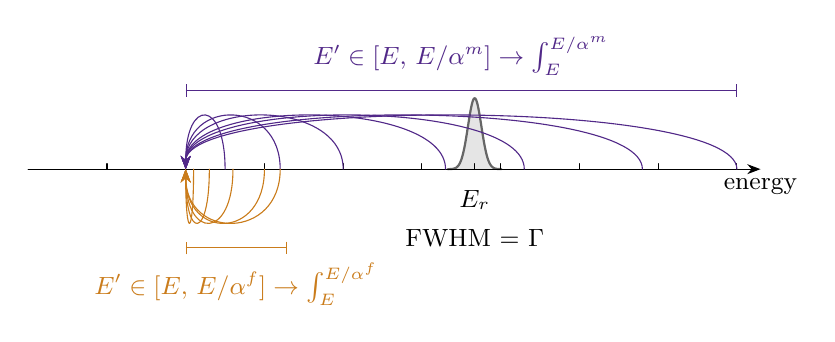
\begin{tikzpicture}[
  >=Stealth, line cap=round, line join=round,
  mod/.style  ={ksupurple, thin},
  fuel/.style ={orange, thin},
  every node/.style={font=\small}
]

% ====================================================================
% DERIVED SETTINGS -- normally no editing is needed below this line.
% The choice keys reject unrecognized variant/profile names.
% ====================================================================
\pgfkeys{
  /sde/variant/.is choice,
  /sde/variant/NR/.code={\pgfmathsetmacro{\GammaUse}{\Gnarrow}},
  /sde/variant/WR/.code={\pgfmathsetmacro{\GammaUse}{\Gwide}},
  /sde/profile/.is choice,
  /sde/profile/Gaussian/.code={\def\drawGaussian{1}\def\drawSLBW{0}},
  /sde/profile/SLBW/.code={\def\drawGaussian{0}\def\drawSLBW{1}},
  /sde/variant/.expanded=\ResonanceVariant,
  /sde/profile/.expanded=\ResonanceProfile
}
\typeout{Slowing-down figure: variant=\ResonanceVariant, profile=\ResonanceProfile, FWHM=\GammaUse}

\pgfmathsetmacro{\EoOverAm}{\Eo/\am}
\pgfmathsetmacro{\EoOverAf}{\Eo/\af}

% Gaussian: Gamma = 2 sqrt(2 ln 2) sigma.
\pgfmathsetmacro{\sigma}{\GammaUse/(2*sqrt(2*ln(2)))}
\pgfmathsetmacro{\xminG}{max(\Emin,\Er-4*\sigma)}
\pgfmathsetmacro{\xmaxG}{min(\Emax,\Er+4*\sigma)}

% SLBW/Lorentzian, shape only: peak height Ares and FWHM GammaUse.
% y(x) = Ares * (GammaUse^2/4) / ((x-Er)^2 + GammaUse^2/4).
\pgfmathsetmacro{\xminL}{max(\Emin,\Er-6*\GammaUse)}
\pgfmathsetmacro{\xmaxL}{min(\Emax,\Er+6*\GammaUse)}

% --- Resonance: fill and outline, behind the scattering arrows ---------
\ifnum\drawGaussian=1
  \path[fill=black!10, draw=none]
    (\xminG,0) --
      plot[domain=\xminG:\xmaxG, samples=181]
        (\x, {\Ares*exp(-((\x-\Er)^2)/(2*\sigma*\sigma))})
    -- (\xmaxG,0) -- cycle;
  \draw[black!60, line width=0.8pt]
      plot[domain=\xminG:\xmaxG, samples=181]
        (\x, {\Ares*exp(-((\x-\Er)^2)/(2*\sigma*\sigma))});
\fi

\ifnum\drawSLBW=1
  \path[fill=black!10, draw=none]
    (\xminL,0) --
      plot[domain=\xminL:\xmaxL, samples=220]
        (\x, {\Ares*(0.25*\GammaUse*\GammaUse)/((\x-\Er)*(\x-\Er)+0.25*\GammaUse*\GammaUse)})
    -- (\xmaxL,0) -- cycle;
  \draw[black!60, line width=0.8pt]
      plot[domain=\xminL:\xmaxL, samples=220]
        (\x, {\Ares*(0.25*\GammaUse*\GammaUse)/((\x-\Er)*(\x-\Er)+0.25*\GammaUse*\GammaUse)});
\fi

% --- Labels and energy axis -------------------------------------------
\node[black, below=4pt] at (\Er,0) {$E_r$};
\node[black, below=4pt] at (\Er,-0.5) {FWHM = $\Gamma$};

\draw[->] (\Emin,0) -- (\Emax+0.3,0) node[below] {energy};
\foreach \x in \TickEnergies \draw (\x,0) -- ++(0,0.07);
\draw (\Er,0) -- ++(0,0.07);

% --- Incoming-energy integration intervals ----------------------------
\draw[ksupurple, |-|]
  (\Eo,\IntervalHeight) -- node[above=2pt, mod]
  {$E' \in [E,\,E/\alpha^{m}] \rightarrow \int^{E/\alpha^m}_E$}
  (\EoOverAm,\IntervalHeight);
\draw[orange, |-|]
  (\Eo,-\IntervalHeight) -- node[below=2pt, fuel]
  {$E' \in [E,\,E/\alpha^{f}]\rightarrow \int^{E/\alpha^f}_E$}
  (\EoOverAf,-\IntervalHeight);

% --- Illustrative scattering arrows -----------------------------------
\foreach \Ep in \ModeratorEnergies
  \draw[mod,->, thin] (\Ep,0)
    .. controls ($(\Ep,0)+(0,\ArcHeight)$)
            and ($(\Eo,0)+(0,\ArcHeight)$) .. (\Eo,0);
\foreach \Ep in \FuelEnergies
  \draw[fuel,->, thin] (\Ep,0)
    .. controls ($(\Ep,0)+(0,-\ArcHeight)$)
            and ($(\Eo,0)+(0,-\ArcHeight)$) .. (\Eo,0);

\end{tikzpicture}
\end{document}
